\chapter{Wellenoptik}

\section{Wiederholung (Schwingungen und Wellen)}

\subsection{Schwingungen}

\folie{Harmonische Schwingungen}\\
\lcom{Zwei grössen: Amplitude und Phase, und zwei komponenten: inphase, und out of phase}

\subsection{Wellen}

\folie{Harmonische ebene Welle, Polarisation, Kugelwellen}\\
Harmonische Ebene Welle in 1D
\begin{equation*}
A(x,t) = A_0 \cos (\omega t - kx + \varphi)= \Re\left[\hat{A} e^{-i(\omega t - kx)}\right]
\end{equation*}
\lcom{Das Minus in der Komplexen Schreibweise Stammt aus der Wellengleichung. Es kommt auch aus der Lorenzinvarianten. }\\
\lcom{Da EM-Wellen Transversalwellen sind und Ladungserhaltung/Eichinvarianz gilt, kann es nur zwei Polarisationsrichtungen geben. }\\
\folie{Wellengleichung}

\subsection{Fourier-Transformation}

\lcom{Ein Thema das nie richtig behandelt wird, aber wichtig ist, vielleicht leiste ich heute ein Beitrag dazu.}\\
Harmonische Schwingungen:
$$A(t) = A_0 \cos (\omega t + \varphi) = \Re [\hat A_0 e^{-i\omega t}]$$
Periodische Schwingungen: Fourier-Reihe
$$A(t) = A(t + T) = \summ{n = 0}{\infty} A_n \cos(m \omega_0 t + \varphi_n) = \Re \left[\summ{n = 0}{\infty} \hat A_n e^{-i n \omega_0 t}\right]$$
$$\omega_m \leq n \omega_0$$
Beliebige Zeitabhängigkeit: Fourier Transformation
$$A(t) = \intt{-\infty}{+\infty} A(\omega) \cos (\omega t + \varphi(\omega)) \dd \omega = \Re \left[\int \hat A (\omega) e^{-i\omega t} \dd \omega \right]$$
Bemerkung: \lcom{Wir können zwei Fourier Transformationen machen, nach Ort und nach Zeit.}
\begin{itemize}
	\item Umkehr Transformation: Faktor $2 \pi$ taucht auf
	\item Analog für $e^{i \vec{k} \vec{x}}$
	\item Die Fourier Transformation impliziert eine ''Unschärfe Relation'' \lcom{Eine Eigenschaft der FT}
		$$\Delta \omega \Delta t \approx \mathcal O(2 \pi) \qquad \Delta \vec{k} \Delta \vec{x} \approx \mathcal O(2\pi)$$
\end{itemize}
\emph{Beispiel:} \textbf{Gedämpfte Schwingung, Zerfall, Relaxation}\\
Exponentielles Abklingverhalten
$$A(t) \propto e^{-\frac{t}{\tau}} \quad \Leftrightarrow \quad \textrm{ = Lorentz-Funktion}$$
$\tau$: Zeitkonstante
\folie{Zeitraum/Frequenzraum}\\
\lcom{Ein exponentieller Zerfall ist immer mit der Lorentz-Funktion verbunden. Eine ungedämpfte harmonische Schwingung: $\tau = \infty$. }\\
\lcom{Eine unendlich langer, unendlich langsamer Schwingung ist im Frequenzraum unendlich scharf. Eine ungedämpfte harmonische Schwingung ist also im Frequenzraum unendlich scharf und wird damit zu einer Dirac-Delta-Funktion mit dem Peak bei der Frequenz der Schwingung. Eine solche Welle ist im Ortsraum überall verteilt.}\\[5pt]
\emph{Beispiel:} \textbf{Wellenpaket}\\
ebene Welle: $E(\vec{x},t) = E_0 e^{-i(\omega t - \vec{k} \vec{x})}$
$$\Rightarrow |E|^2 = E_0^2 = \const$$
\folie{Wellenpakete}\\
\lcom{Im Wellenvektorraum ist die Welle jedoch wieder mit einer Delta-Funktion beschrieben. Ein Wellenpaket ist im Ortsraum lokalisiert aber im Wellenvektorraum sehr unscharf verteilt.}\\
\lcom{Die Fouriertransformation einer Gauß-Verteilung (wird oft für Wellenpakete verwendet) ist wieder eine Gauß-Verteilung. Die Fouriertransformation einer Exponentiell Abfallenden Welle ist eine Lorenz-Funktion.}

\subsection{Kohärenz}

\begin{description}
	\item[Definition:] Zwei oder mehr Wellen sind Kohärent, wenn die Zeitabhängigkeit der Auslenkungen bis auf eine Phasendifferenz der gleiche ist \mau
\end{description}
Viele gründe warum Wellen nicht kohärent sind:
\begin{itemize}
	\item spontan emittiertes Licht vieler unabhängiger Lichtemmiter (heiße Atome)
	\item zwei Lichtquellen schwanken leicht in Frequenz Amplitude, Phase (nicht stabil)
	\item zu ausgedehnte Lichtquelle
\end{itemize}
Gegenbeispiele:
\begin{itemize}
	\item stimulierte Emission: einfallendes Licht zwingt angeregte Atome synchron mit dem Lichtfeld zu Schwingen und abzustrahlen.
\end{itemize}
\textbf{Kohärenzlänge:}\\
\lcom{Kohärenzlänge: Keine Lichtquelle kann unendlich kohärentes Licht erstellen. Die minimal unterschiedlichen Frequenzen sorgen dafür, dass das Licht nach einer Weile nicht mehr kohärent ist. Die Flugweite der Lichtstrahlen bis die Kohärenz nicht mehr gegeben ist, nennt man Kohärenzlänge.}\\
\textbf{Kohärenzzeit:}\\
\lcom{Die dauer in der Kohärentes Licht nicht nicht mehr kohärent wird nennt man Kohärenszzeit. }
Kohärenzzeit = Kohärenzlänge/$c$

\noindent
\textbf{Experimente:}
\begin{enumerate}[(i)]
	\item Licht mit genügend großer Kohärenzlänge
	\item Licht aus \textbf{einer} Quelle aufteilen, wenn mehrere Kohärente Strahlen benötigt werden.
\end{enumerate}


% Vorlesung 13.11.18

\section{Inteferenz und Beugung I}

\subsection{Inteferenz am Doppelspalt}

Berechnung der Maxima und Minima ($ d $ ist der Abstand der Spalte)
\begin{description}
	\item[Gangunterschied] $x = d \sin \alpha$
\end{description}
Maxima wenn $x$ ein Vielfaches von $\lambda$ ist (konstruktive inteferenz)
\begin{itemize}
	\item[$\rightarrow$] $x = n \lambda$
	\item[$\Rightarrow$] Maxima: $\sin\alpha = n \frac{\lambda}{d}$
	\item[$\Rightarrow$] Minima: $\sin\alpha = \left(n + \frac{1}{2}\right)\frac{\lambda}{d}$
\end{itemize}
Triviale aber Wichtige Feststellung: nicht nur $d$, nicht nur $\lambda$, sondern $\frac{\lambda}{d}$\\
\emph{Bemerkung: } $$k= \frac{2\pi}{\lambda}$$
$$\Rightarrow \quad kx = 2 \pi n$$
$$\Delta f = 2\pi n = kx = \frac{2 \pi}{\lambda}x$$
Feststellung: Ortsraum $k$-Raum reziprok 
%
%
%
% f = varphi a ? = alpha
%
%
%
\subsection{Beugung am Einzelspalt}

Brechung der Intensitätsverteilungen $ I(\alpha) $, in 6 Schritten

\begin{enumerate}[(1)]
	\item Strahl über Spalt wird in $ N $ Teilstrahlen zerlegt im Abstand: $ \Delta b = \frac{b}{N} $
	\item Amplitude eines Teilstrahls $ a = \frac{\sqrt{I_0}}{N} $
	\item Gangunterschied benachbarter Strahlen: $ x = \Delta b \sin \alpha $
	\item Phasenunterschied benachbarter Strahlen: $ \Delta \varphi = k x = k \Delta b \sin \alpha  $
	\item Gesamtamplitude $ \widehat{=} $ Summe der $ N $ Teilstrahlen
	\begin{equation*}
	\Rightarrow \quad A = a \sum_{n=0}^{N-1} e^{-i(\omega t + f_n)} = a e^{-i \omega t} \sum_{n=0}^{N-1} e^{i n \Delta \varphi}
	\end{equation*}
	$ f_n $ ist die Phase des $ n $-ten Teilstrahls und $ f_n = n \cdot \Delta \varphi $
	\begin{equation*}
	A = a e^{-i\omega t} \frac{e^{i N \Delta \varphi}-1}{e^{i \Delta \varphi}-1} = a e^{- i \omega t} e^{i \frac{N \Delta \varphi}{2}} \frac{\sin\left(\frac{N}{2} \Delta \varphi\right)}{\sin\left(\frac{1}{2} \Delta \varphi\right)}
	\end{equation*}
	\begin{equation*}
	\Rightarrow \quad I(\alpha) = A^2 = a^2 \frac{\sin^2\left(\frac{N}{2} \Delta \varphi \right)}{\sin^2 \left(\frac{1}{2} \Delta \varphi \right)} = a^2 \frac{\sin^2 (x)}{\sin^2 \left(\frac{x}{N}\right)} \qquad x \defeq \pi \frac{b}{\lambda} \sin \alpha
	\end{equation*}
	\item Grenzübergang $ \Delta b \rightarrow 0 $ oder $ N \rightarrow \infty $:
	\begin{equation*}
	\Rightarrow \quad \sin^2\left(\frac{x}{N}\right) = \frac{x^2}{N^2}
	\end{equation*}
	\begin{equation*}
	\Rightarrow \quad I(\alpha)  = N^2 a^2 \frac{\sin^2(x)}{x^2}
	\end{equation*}
	\textbf{Lösung:}
	\begin{equation*}
	\rmbox{I(\alpha) = I_0 \frac{\sin^2(x)}{x^2}} \qquad x \defeq \pi \frac{b}{\lambda} \sin \alpha
	\end{equation*}
\end{enumerate}
\textbf{Diskussion:}\\[5pt]
Hauptmaxima: $ x = 0 \quad \rightarrow \quad \alpha = 0 $\\
Minima: $ \sin x = 0 \quad \rightarrow \quad x = n \pi \quad \Rightarrow \quad \sin \alpha = n \frac{\lambda}{b} $\\
Nebenmaxima: $ |\sin x| = 1 \quad \rightarrow \quad x = \left(n + \frac{1}{2}\right) \pi \quad \Rightarrow \quad  \sin \alpha = \left(n + \frac{1}{2}\right) \frac{\lambda}{b} $\\[5pt]
\lcom{Die Gleichungen sind unabhängig vom Abstand des Schirms. Dies stammt aus der Annahme es handelt sich um Ebene Wellen,die es nur die nur im Fernbereich gibt. Daher gelten unsere Gleichungen und Annahmen auch nur im Fernbereich. Ist der Abstand zum Schirm nicht Wesentlich größer als die Spaltbreite oder der Abstand der Spalten, gelten sie nicht mehr. Mehr dazu im Abschnitt Interferenz und Beugung II.}\\[5pt]
ACHTUNG:\\
Implizit Annahme ebener Wellen $ \Rightarrow $ Rechnung nur richtig im Fernbereich \mau

\subsection{Beugung am Gitter}

\textbf{Definition:}\\
Gitter: Regelmäßige Anordnung von ,,Strichen``
\folie{Licht am optische Gitter} (wieder Annahme ebener Wellen)\\
Brechungs
\begin{enumerate}[(1)]
	\item Überlagerung von $ N $ Strahlen im Abstand $ d $
	\item Amplitude eines Strahls $ a = \sqrt{I_0} $
	\item Gangunterschied von benachbarten Strahlen $ x = d \sin \alpha $
\end{enumerate}	
Weiter wie beim Einzelspalt:
\begin{enumerate}[(4)]
	\item[(4)] Phasenunterschied $ \Delta \varphi = k x = k d \sin \alpha $
	\item[(5)] Gesamtamplitude $ \widehat{=} $ Summe der Teilstrahlen
	\begin{equation*}
	\Rightarrow \quad A = a e^{-i \omega t} \sum_{n=0}^{N-1} e^{i n \Delta \varphi}
	\end{equation*}
	\begin{equation*}
	\Rightarrow \quad A(\alpha) = A_0 \frac{\sin \left(\pi \frac{N d}{\lambda} \sin \alpha \right)}{\sin \left( \pi \frac{d}{\lambda} \sin \alpha \right)} \qquad A_0: \tx{ geeignet definiert}
	\end{equation*}
	\begin{equation*}
	I(\alpha) = A^2
	\end{equation*}
	\folie{Interferenzmuster in Abhängigkeit der Spaltenzahl}
\end{enumerate}
\textbf{Diskussion:}\\[5pt]
Hauptmaxima: Nenner klein $ \pi \frac{d}{\lambda} \sin \alpha = m \pi $
\begin{equation*}
\Rightarrow \qquad \sin \alpha = m \frac{\lambda}{d}
\end{equation*}
Nebenmaxima: Zähler klein $ \Rightarrow \pi \frac{N d}{\lambda} \sin \alpha = m \pi $
\begin{equation*}
\Rightarrow \qquad \sin \alpha = m \frac{\lambda}{N d}
\end{equation*}
Breite der Hauptmaxima:\\
Verhält sich wie der Abstand benachbarter Nebenmaxima
\begin{equation*}
\Rightarrow \qquad B = \frac{2 \lambda}{N d}
\end{equation*}
Dispersion der Hauptmaxima ($ \lambda $ bzw. $ \omega $ Abhängigkeit)\\
Lage: $ \sin \alpha = m \frac{\lambda}{d} $
\begin{equation*}
\Rightarrow \quad \frac{\dd \alpha}{\dd \lambda} = \frac{m}{d} \arccos \alpha \quad \Rightarrow \quad \frac{\dd \alpha}{\dd \lambda} > 0
\end{equation*}
\lcom{Wenn ihr eine scharfe Linie wollt sollte euch sofort Gitter einfallen. }

\subsection{Beugung am Raum- oder Oberflächengitter}

\textbf{Definition:}\\
Raumgitter: Kristall $ \widehat{=} $ regelmäßige Anordnung von Atomen im 3D Raum\\
\folie{Diamant Kristallgitter}
\begin{equation*}
\Rightarrow \quad \rmbox{2 d \sin \alpha = m \lambda} \qquad \tx{Bragg-Bedingung}
\end{equation*}
$ d $ ist der Abstand von zwei Kristall-Ebenen oder Netzebenen\\
\versuch{Doppelspalt}
% unten angstöm ändern evtl OK DONE -az
\noindent
Typischer Zahlenwert:
\begin{equation*}
d \approx 1 \, \tx{\AA} \quad \Rightarrow \quad \lambda \approx 1 \,  \tx{\AA} \quad \approx \quad \tx{Röntgenstrahlung oder X-Ray}
\end{equation*}
\versuch{Gitter}
\versuch{Kristall Struktur Messung it Röntgenstrahlung}
Anwendung von Kristallen: Röntgenstrukturanalyse mittels Röntgendefraktometer\\
X-Ray: \lcom{Die Wechselwirkung von Röntgenstrahlung mit Materie ist die mit den Elektronen also der Lorenz-Lorentz-Oszillator $ \vec{F} = q \vec{E} $. Die Röntgenstrahlung Wechselwirkt also mit den Ladungen. Was wir beobachten ist also die Lage der Elektronen also nur indirekt die Lage der Atome.}

% Vorlesung 14.11.18 (10)
% andrez comment 1 %% mehr lügen! hier gibts keine kommentare -az

\noindent
\emph{Beispiel:} \textbf{Srukturanalyse von Kristallen}

\begin{itemize}
	\item X-ray: $ \vec{F} = q \vec{E} $
	\begin{itemize}
		\item Streuung an der Elektronenhülle
		\item Bestimmung der Elektronenladungshülle
	\end{itemize}
	\item Neutronen $n$: starke WW
	\begin{itemize}
		\item Streuung am Kern
		\item Bestimmung der Kernpositionen
	\end{itemize}
	\item Spin: magnetische Dipol-Dipol-WW
	\begin{itemize}
		\item Streuung an Elektronenspins
		\item $ \Rightarrow $ Magnetismus
	\end{itemize}
\end{itemize}
\lcom{Wie gut kommen Elektronen durch material durch? Überhaupt nicht gut, bei Isolatoren ist es in dem sehr kleinen 0,000... \AA \ Bereich, bei Metallen trifft das Elektron gleich auf den ''Elektronen See''.}\\[10pt]
\emph{Beispiel:} \textbf{Untersuchung von Oberflächen LEED} (Low Energy Electron Diffraction)

\begin{itemize}
	\item $ e^- $:
	\begin{itemize}
		\item Streuung an der Elektronenhülle
		\item Eindringtiefe $ \approx 100 \, \tx{\AA} \Rightarrow $ Oberflächenanalyse
	\end{itemize}
\end{itemize}
\lcom{Die \textbf{Energie von Raumtemperatur} ist ungefähr $ \frac{1}{40} \, \tx{eV} $. Sollte man Wissen.}\\
\folie{zu LEED}

\subsection{Interferenz an planparallelen Glasplatten}

\folie{zu Reflexion an einer Glasplatte}\\
\begin{center}
	\centering
	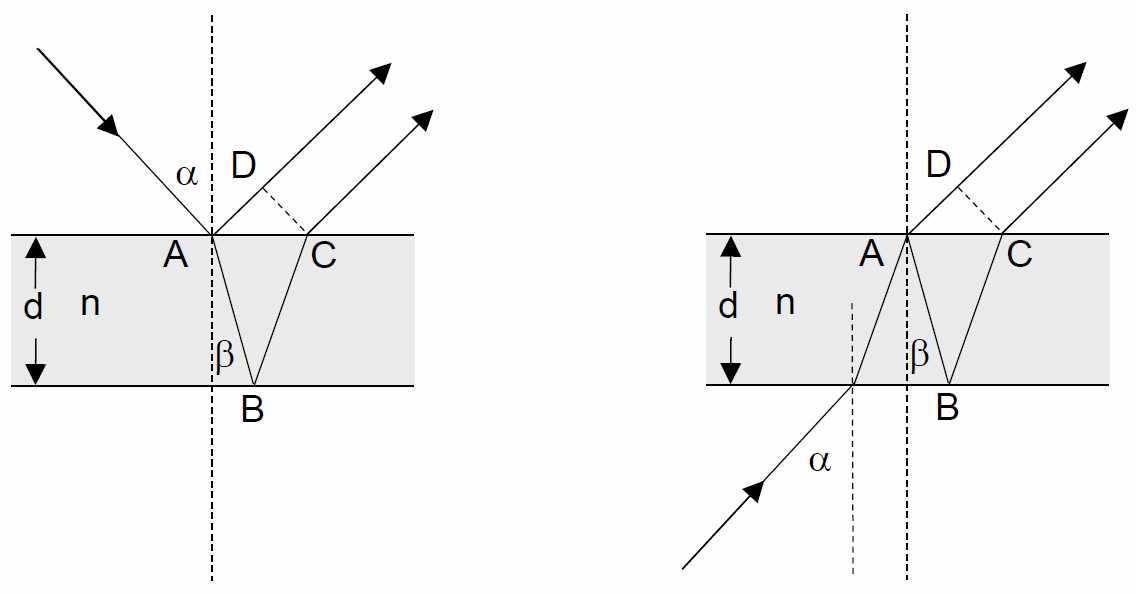
\includegraphics[width=0.6\textwidth]{Abbildungen/Glasplatten.png}
\end{center}

\subsubsection{Reflexion}

\begin{enumerate}[(1)]
	\item Länge der Wege $ \ol{AB} $ und $ \ol{BC} $
	\begin{equation*}
	x_{AB} = \frac{d}{\cos \beta} \quad x_{BC} = \frac{d}{\cos \beta}
	\end{equation*}
	\item Weg $ \ol{AD} $
	\begin{equation*}
	x_{AD} = \ol{AC} \sin \alpha = 2 d \tan \beta \sin \alpha
	\end{equation*}
	\item Gangunterschied
	\begin{equation*}
	x = n \left(x_{AB} + x _{BC}\right) - x_{AD}
	\end{equation*}
	$ n $: Brechungsindex der Glasplatte\\
	mit $ \sin \alpha = n \sin \beta $ gilt:
	\begin{equation*}
	x = 2 d n \cos \beta = 2 d \sqrt{n^2 - \sin^2 \alpha}
	\end{equation*}
	\item Phasenunterschied\\
	Phasenunterschied aufgrund des Gangunterschieds $ \Delta \varphi = kx = \frac{2\pi}{\lambda} x $\\
	$ \approx $ senkrechter Einfall:\\
	Phasensprung um $ \pi $ bei der Reflexion am optisch dichteren Medium \color{red!75!black} \mau \color{black}\\
	\lcom{Bei senkrechtem Einfall, bei der Reflexion an einem optisch dichteren Medium, tritt
	ein Phasensprung um $ \pi $ auf (dies ergibt sich aus den Randbedingungen siehe z.B. ExpII, ist
	ähnlich zur Reflexion an ,,harter`` Oberfläche, siehe ExpI)}
	\begin{equation*}
	\Rightarrow \Delta \varphi = k x  + \pi
	\end{equation*}
	\item Für konstruktive Interferenz (Maxima): $ \Delta \varphi = m 2 \pi $
	\begin{equation*}
	\Rightarrow \qquad 2 d \sqrt{n^2 - \sin^2 \alpha} = \left(m + \frac{1}{2}\right) \lambda
	\end{equation*}
\end{enumerate}

\subsubsection{Transmission}

\begin{enumerate}[(1)]
	\item Gangunterschied wie zuvor
	\begin{equation*}
	x = n (x_{AB} + x_{BC}) - x_{AD} = 2 d \sqrt{n^2 - \sin^2 \alpha}
	\end{equation*}
	\item Phasenunterschied\\
	Gangunterschied $ \Rightarrow \Delta \varphi = kx $\\
	Phasensprünge $ \Rightarrow 0 $
	\begin{equation*}
	\Rightarrow \qquad \Delta \varphi = kx
	\end{equation*}
	\item Maxima:
	\begin{equation*}
	\Rightarrow \qquad 2d\sqrt{n^2 - \sin^2 \alpha} = m \lambda
	\end{equation*}
\end{enumerate}
\textbf{Test:}\\
Annahme: keine Absorption in der Glasplatte: \lcom{Die Intensitäten der Reflexion und die der Streuung sollten sich zu Gesamtintensität aufsummieren. }
\begin{equation*}
\Rightarrow \tx{ zu erwarten: } \quad I = I_{\tx{reflektiert}} + I_{\tx{transmittiert}}
\end{equation*}
Wie erwartet da wo die Transmission maximal ist ist die Reflexion minimal und umgekehrt. Immer um $ \frac{\lambda}{2} $ verschoben.
\subsubsection{Anwendung}
\begin{itemize}
	\item \versuch{Interferenz mit zwei angewinkelten Spiegeln Fres'nelscher Doppelspiegel}
	\folie{Fres'nelscher Doppelspiegel}
	\item \folie{Newton's Ringe}
	\item \versuch{Seifenblase} die in Regenbogenfarben schillert
	\item \versuch{Interferenz an Planparalleler Folie} (mit grünem Laserlicht demonstriert)
\end{itemize}

\subsection{Vielstahlinterferenz, Fabry-P\'erot-Interferometer}

\folie{Vielstrahlinterferenz an Planparallelen Platten}
\begin{center}
	\centering
	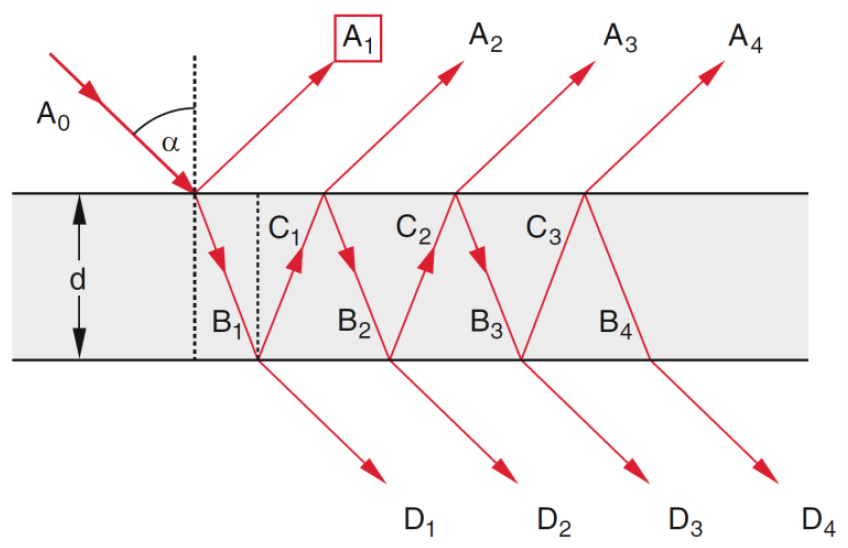
\includegraphics[width=0.6\textwidth]{Abbildungen/Glasplatten2.png}
\end{center}
\lcom{Die Interferenz ähnelt der bei einem Gitter. Der große Unterschied liegt darin, dass die Intensität der Teilstrahlen mit zunehmenden Reflexionen abnimmt. }\\
Reflexion (Transmission aus $ I = I_{\tx{ref}} + I_{\tx{trans}} $)
\begin{enumerate}[(1)]
	\item Intensitäten der jeweiligen Teilstrahlen berücksichtigen\\
	$ \Rightarrow $ Reflexionskoeffizient $ R $
	\begin{align*}
	|A_1| &= \sqrt{R} |A_0|\\
	|B_1| &= \sqrt{1 - R} |A_0|\\
	|D_1| &= \sqrt{1-R} |B_1| = (1-R) |A_0|\\
	|C_1| &= \sqrt{R} |B_1| = \sqrt{R}\sqrt{1 - R} |A_0|\\[7pt]
	|A_2| &= \sqrt{1 - R} |C_1|\\
	|B_2| &= \sqrt{R} |C_1| = R \sqrt{1 - R} |A_0|
	\end{align*}
	Einsetzen liefert\\
	$\Rightarrow \quad |A_{m+1}| = \sqrt{1-R} |C_m| = \sqrt{1-R} \sqrt{R} |B_m| = \sqrt{1-R} \sqrt{R} \sqrt{R} |C_{m-1}| = R |A_m|$
	\vspace{5pt}
	\begin{equation*}
	\Rightarrow \qquad |A_{m+1}| = R |A_m| \qquad |D_{m+1}| = R |D_m|
	\end{equation*}
	\item Gangunterschied benachbarter Strahlen (siehe Platte)
	\begin{equation*}
	x = 2d \sqrt{n^2 - \sin^2 \alpha} 
	\end{equation*}
	\item Phasenunterschied
	\begin{equation*}
	\Delta \varphi = \custo{\leftarrow}{kx}{\mathclap{\tx{Gangunterschied}}} + \tx{Phasensprünge}
	\end{equation*}
	Bei den Phasensprüngen folgt nach längerer Arbeit, dass nur der Phasensprung $ A_1 $ übrig bleibt.
	\item Gesamtamplitude
	\begin{equation*}
	A = \color{red} \pm \color{black} \sum_{m=1}^{N} A_m e^{i(m-1) \Delta \varphi}
	\end{equation*}
	$ N $: Anzahl der betrachteten Teilstrahlen\\
	$ \color{red} \pm \color{black} $: Berücksichtigt die Phasensprünge
	\item Grenzübergang $ N \to \infty $ (unendlich lange Glasplatte):
	\begin{equation*}
	\Rightarrow \qquad A = \pm A_0 \sqrt{R} \frac{1 - e^{i \Delta \varphi}}{1 - R e^{i \Delta \varphi}}
	\end{equation*}
	\begin{equation*}
	\Rightarrow \rmbox{I_R = |A^2| = 2 I_0 R \frac{1 - \cos \Delta \varphi}{1 - 2 R \cos \Delta \varphi + R^2}}
	\end{equation*}
\end{enumerate}

\subsubsection{Ergebnis}

\begin{center}
	\begin{minipage}{.6\linewidth}
		\frbox{Airy-Formeln}{
			\begin{equation*}
			I_R = I_0 \frac{F \sin^2 \left(\frac{\Delta \varphi}{2}\right)}{1 + F \sin^2\left(\frac{\Delta \varphi}{2}\right)}
			\end{equation*}
			\begin{equation*}
			I_T = I_0 \frac{1}{1 + F \sin^2 \left(\frac{\Delta \varphi}{2}\right)}
			\end{equation*}
		}
	\end{minipage}
\end{center}
\begin{equation*}
F = \frac{4 R}{(1-R)^2} \qquad \frac{\Delta \varphi}{2} = 2 \pi \frac{d}{\lambda} \sqrt{n^2 - \sin^2 \alpha}
\end{equation*}
\emph{Beispiel:} \textbf{senkrechter Einfall}
\begin{equation*}
\Rightarrow \alpha = 0 \qquad I_T = I_0 \frac{1}{1 + F \sin^2 (n d k)}
\end{equation*}
wobei $ k = \frac{2 \pi}{\lambda} $
Maxima: $$ 2 n d = m \lambda $$
FWHM (full width at half maximum)
$$ \epsilon = 4 \arcsin\sqrt{\frac{1}{F}} \approx \frac{4}{\sqrt{F}} $$
$ \Rightarrow \quad  R \to 1 \ \Leftrightarrow $ schmal-bandige Maxima\\
\folie{Maxima beim FWHM}\\[5pt]
\textbf{Anwendung: Fabry-P\'erot-Interferometer}\\
\folie{zu Fabry-P\'erot-Interferometern}\\[5pt]
\versuch{Natrium-Dampf-Lampe Interferenz}
\folie{Interferenz mit einer Natrium-Dampf-Lampe}\\[5pt]
\versuch{Abpumpen der Luft beim Interferenzmuster der Natrium-Dampf-Lampe}
\lcom{Das Muster verändert sich erheblich obwohl der Unterschied der Brechungsindizes so gering war. Also hat das Farbinterferometer eine sehr hohe Auflösung. }

% Vorlesung %20.11.18

\section{Interferenz und Beugung II - Huygen'sches Prinzip}

\subsection{Huygen'sches Prinzip}

\rbox{Jeder Punkt einer Wellenfront ist Ausgangspunkt einer neuen Elementarwelle.}
\noindent
\emph{Beispiel:} \textbf{Brechung}\\
Erklärung über Ausbreitung ebener Wellen \folie{Brechung mit Ebenen Wellen}
%
%
%
% Bild von Folie
%
%
%
\subsection{Interferenz am Doppelspalt}

Jeder Spalt, wenn er klein genug ist, wird als ,,Sender`` einer Elementarwelle angesehen.\\
$ \Rightarrow $ Überlagerung von zwei Kugelwellen.\\
\folie{zu Doppelspalt mit Kugelwellen}
%
%
%
% Bild von Folie einfügen
%
%
%
\subsection{Beugung}

Beugung bezeichnet das Phänomen, das Licht (und andere Wellen) in Bereiche vordringt, in welche es als Strahl betrachtet nicht vordringen dürfte.\\
\lcom{Beugung tritt immer an Stellen auf, an denen die Transmission einer Welle verhindert wird. Dies ist z.B. der Fall an Kanten bei denen an einer Seite komplette Abschattung und an der anderen komplette Transmission stattfindet.}\\
\lcom{Interferenz tritt dann auf, wenn es zwei solche Stellen gibt an denen Beugung auftritt.}\\
\versuch{Laser mit Kante und später Loch-/Kreisblende und später Stecknadelkopf}
\lcom{Man sieht auch ein dieser einzelnen Kante Interferenz. Dies zu verstehen ist Ziel der heutigen Vorlesung. \textbf{Das Interferenzmuster ist die Fouriertransformation einer Stufenfunktion.} Bei der Lochblende einer Fouriertransformation eines ,,Loches``.}\\
\folie{Doppelspalt Beugung} \folie{Einzelspalt}\\

\subsection{Allgemeine Behandlung der Beugung}

\lcom{Zur Verallgemeinerung Behandeln wir nun das Kirchhoff'sche Beugungsintegral.}

\subsubsection{Kirchhoff'sches Beugungsintegral}

\lcom{In verschiedenen Büchern treten häufig andere Formel des Gleichen Integrals auf.}\\
\folie{Beugungsintegral}\\
\lcom{Die Blende wird als eine Transmissionsfunktion beschrieben. Zu jedem Punkt aus dem Schirm gibt es dann ein Integral der Intensitäten aller Elementarwellen aus der Blende.}
%
%
%
% Bild einfügen
%
%
%
\noindent
Blendenöffnung bei $ z = 0 $\\
Beobachtungsschirm bei $ z = z' = z_0 $
\frbox{Kirchhoff'sches Beugungsintegral}{
\begin{equation*}
\vec{E}(\vec{x}') = \frac{ik}{2 \pi} \int Q \tau(x,y) \vec{E}_{\tx{ein}} (\vec{x}) \frac{e^{-ikr}}{r} \dd \sigma 
\end{equation*}}

\noindent
$ Q \defeq $ Neigungsfaktor\\
$ \tau \; \defeq $ Transmissionsfunktion mit $ \left\{ \begin{array}{ll}
\tau = 1 : & \tx{vollständige Transmission} \\ \tau = 0 : & \tx{undürchlässig}
\end{array} \right. $\\
$ r \ \defeq $ Abstand des Punkts $ \vec{x} $ und $ \vec{x}' $
\begin{equation*}
r^2 = (\vec{x} - \vec{x}')^2 = (x-x')^2 + (y-y')^2 + z'^2
\end{equation*}
\textbf{Sketch der Herleitung}
\begin{enumerate}[(1)]
	\item Für das von der Blende bei $ z = 0 $ durchgelassene Licht gilt:
	\begin{equation*}
	E_{\tx{Blende}} (x,y) = E_{\tx{ein}} (x,y,z=0) e^{i\varphi (x,y,z=0)}
	\end{equation*}
	\item Jeder Punkt der Öffnung erzeugt eine Elementarwelle
	\begin{equation*}
	\dd E(x',y',z') \propto Q \tau(x,y) E_{\tx{ein}} (x,y) \frac{e^{-ikr}}{r} \ub{\dd x \dd y}_{d\sigma}
	\end{equation*}
	\begin{equation*}
	Q \propto \frac{1}{2} (\cos \theta_1 + \cos \theta)
	\end{equation*}
	\item Insgesamt:
	\begin{equation*}
	E(x,y',z') \propto \int Q \tau(x,y) E_{\tx{ein}} \frac{e^{-ikr}}{r} \dd \sigma
	\end{equation*}
	\item  Vektoren und Beträge ,,richtig```machen.
\end{enumerate}
\textbf{Grenzfälle:}
\begin{itemize}
	\item Frauenhofer-Beugung:\\
	Abstand des Schirms von der Blende sehr groß gegenüber Öffnung der Blende.
	\begin{equation*}
	z' \gg x,y \qquad z_0 \gg \frac{b^2}{\lambda}
	\end{equation*}
	\item Fresnel Beugung:\\
	Abstand des Schirms von Blende klein.
	\begin{equation*}
	z' \ll x,y \qquad z_0 \ll \frac{b^2}{\lambda}
	\end{equation*}
	\item Überganszone $ z_0 \approx \frac{b^2}{\lambda} $
\end{itemize}
\folie{Folie Nah-/Übergangs-/Fernbereich}

\subsection{Allgemeines Ergebnis für die Beugung im Fernbereich, Frauenhofer Beugung}

Fernbereich: $ z' \gg x,y $
\begin{equation*}
r = \sqrt{(x-x')^2 + (y-y')^2 + z'^2}
\end{equation*}
\lcom{Zur Näherung: Näherungen zu machen ist nicht sehr einfach und der Prozess nicht sehr präzise zu Beschreiben. Es ist nicht leicht eine gute Näherung zu finden. Man muss dabei darauf Achten, dass man durch seine Näherung nicht interessante physikalische Zusammenhänge ,,Wegnähert``. In unserem Fall muss die $ e $-Funktion genau genähert werden, das r im Nenner nur grob.}\\
präziser Nähern wir $ z' \gg \frac{1}{\lambda} (x^2 + y^2) $
\begin{equation*}
r \approx z' \left(1 - \frac{xx'}{z'^2} - \frac{yy'}{z'^2} + \frac{x'^2 + y'^2}{2 z'^2}\right)
\end{equation*}
Im Nenner $ r \approx z' $\\
In dieser Näherung auch $ Q \approx 1 $

\subsubsection{Beugungsintegral für Frauenhofer Beugung}

Nebenrechnung: $ \frac{e^{-ikr}}{r} \approx \frac{e^{-ikz'}}{z'} e^{ik\frac{x'}{z'}x} e^{ik\frac{y'}{z'}y} e^{-ik \frac{1}{2 z'} (x'^2 + y'^2)} $\\
Die ersten Beiden Faktoren hiervon landen später im Vorfaktor $ A $.
\begin{equation*}
\vec{E}(\vec{x}') = \ub{A(\vec{x}')}_{\mathclap{\substack{\tx{alles Lästige} \\ \tx{geht dort rein}}}} \int \tau(x,y) \vec{E}_{\tx{ein}}(x,y) e^{i k \frac{x'}{z'} x} e^{ik\frac{y'}{z'}y} \dd x \dd y
\end{equation*}
2D Fourier Integral:
\begin{equation*}
\vec{F} (u,v) \equiv \int \tau(x,y) \vec{E}_{\tx{ein}} (x,y) e^{iux} e^{ivy} \dd x \dd y
\end{equation*}
\frbox{Beugungsintegral für Frauenhofer Beugung}{
\begin{equation*}
\Rightarrow \quad \vec{E}(\vec{x}') = A(\vec{x}') \vec{F} \left(k \frac{x'}{z'} , k \frac{y'}{z'}\right)
\end{equation*}}
\noindent
\emph{Beispiel:} \textbf{Einfachspalt}
\begin{align*}
\tx{Ortsraum} \qquad &\Leftrightarrow \qquad \tx{Fourier Raum}\\
\tau(x,y) = \casess{1}{\forall  \frac{-b}{2} \le x \le \frac{b}{2}}{0}{\tx{sonst.}} \qquad &\Leftrightarrow \qquad \vec{F}(k) = \frac{\sin x}{x} \qquad x = \frac{\pi}{b} k \frac{x'}{z'}\\
\tx{schmaler/breiter Spalt} \qquad &\Leftrightarrow \qquad \tx{breites/schmales Interferenzmuster}
\end{align*}
\begin{equation*}
\Delta x \Delta h < \const
\end{equation*}

\subsection{Auflösungsvermögen optischer Instrumente}

\lcom{Es ist Wichtig zu Wissen von welcher Art von Vergrößerung geredet wird. Welche wir hier benutzen wird später genauer erklärt.}

\subsubsection{Lochkurven}

\folie{Zu Lochkurven und Darstellung mit Lochblenden}\\
\versuch{Darstellung von Dia mit Lochblende}

\subsubsection{Rayleigh Kriterium}

\rbox{Zwei Punkte sind gerade dann noch unterscheidbar, wenn das Beugungsmaximum des einen Punktes in das 1.-te Beugungsminimum des anderen Punktes fällt.}
\noindent
\folie{Auflösung: Überlagerung von Beugungsmustern}\\
\lcom{Diese Definition ist nichts eindeutiges. Es ist nur eine Möglichkeit an einem Breiten Übergang von Scharf bis Unscharf.}

\subsubsection{Ein anderes Kriterium}
Abstand der Hauptmaxima muss größer sein als deren Halbwertsbreite.

% Vorlesung %21.11.18

\subsection{Räumliches Auflösungsvermögen}

\emph{Beispiel:} \textbf{Linse}\\
\folie{Zu Bündelung von Licht mit einer Linse}\\[5pt]
\versuch{Laser: Beugung an der Doppellochplatte}
\lcom{Je näher die Löcher in der Blende zueinander rücken, desto ausgeprägter wird das Interferenzmuster.}\\
Beugung an einer Lochblende:\\
1. Maximum:
\begin{equation*}
r \sin \alpha = 0{,}61 \lambda
\end{equation*}
\textbf{Auflösung einer Lochblende}
\begin{equation*}
\Rightarrow \quad \sin \alpha_{\tx{min}} = 1{,}22 \frac{\lambda}{D}
\end{equation*}
$ D: $ Durchmesser des Lochs\\[5pt]
\textbf{Auflösung einer Linse}
\begin{equation*}
\Rightarrow \quad \sin \alpha_{\tx{min}} = 1{,}22 \frac{\lambda}{D}
\end{equation*}
$ D: $ Durchmesser der Linse\\[5pt]
\textbf{Auflösung eines Fernrohrs}\\
Das durch das Objektiv erzeugte Zwischenbild ist bereits beugungsverbreitert.
\begin{equation*}
\Rightarrow \quad \sin \alpha_{\tx{min}} = 1{,}22 \frac{\lambda}{D}
\end{equation*}
$ D: $ Durchmesser des Objektivs\\[5pt]
\textbf{Auflösung eines Mikroskops}\\
Im Unterschied zu vorher ist das einfallende Licht nicht parallel.\\
\folie{zur Auflösung am Mikroskop}
\begin{enumerate}[(1)]
	\item mit der Kleinwinkelnäherung gilt:
	\begin{equation*}
	d = b \alpha_{\tx{min}}
	\end{equation*}
	\begin{align*}
	\Rightarrow \alpha_{\tx{min}} &= 1{,}22 \frac{\lambda}{D} \\
	\Rightarrow \quad \: \, d &= 1{,}22 \frac{b \lambda}{D}
	\end{align*}
	$ D: $ Durchmesser des Objektivs
	\item Für den Abstand $ \delta_x $ \textbf{vor} dem Objektiv gilt
	\begin{equation*}
	\delta_x \approx \frac{f_1}{b} d = 1{,}22 \frac{f_1 \lambda}{D}
	\end{equation*}
	\item Öffnungswinkel $ \varphi $
	\begin{equation*}
	\sin \varphi \approx \frac{D}{2 f_1}
	\end{equation*}
\end{enumerate}
\begin{center}
	\begin{minipage}{.5\linewidth}
		\frbox{Auflösung eines Mikroskop}{
		\begin{equation*}
		\delta_x \approx 0{,}61 \, \frac{\lambda}{n \sin\varphi}
		\end{equation*}	
		}
	\end{minipage}
\end{center}
$ n \sin \varphi : $ numerische Apertur\\
\lcom{Der \textbf{Gültigkeitsbereich der Formel} ist der \textbf{Fernbereich} (Frauenhofer Beugung). Wir versuchen Bessere Ergebnisse zu erzielen indem wir Situationen Betrachten, die außerhalb dieses Gültigkeitsbereichs liegen.}\\
\lcom{Warum tritt der Faktor $ \sin \varphi $ auf? Dies ergibt sich einsichtig aus Abbe's Theorie: Zwei Punkte senden interferierende Kugelwellen aus (siehe Doppelspalt), wobei mindestens das 1.te Nebenmaximum vom Objektiv noch erfasst werden muss, um ein Bild entstehen zu lassen. Daher:}
\begin{equation*}
\tx{1.tes Nebenmaximum: } \sin \alpha = \frac{\alpha}{\delta_x} \Rightarrow \sin \varphi \approx \sin \alpha \Rightarrow \delta_x \approx \frac{\lambda}{\sin \varphi}
\end{equation*}

\noindent
\textbf{Verbesserungen} der beugungsbegrenzten Auflösung:
\begin{itemize}
	\item kleines $ \lambda $
	\begin{itemize}
		\item[$ \rightarrow $] Elektronenmikroskop ($ 1 \, \tx{nm} $)
		\item[$ \rightarrow $] Röntgen (in Entwicklung)
	\end{itemize}
	\item Immersionsöl mit Brechungsindex von $ n \approx 1{,}5 $
	\item Nahfeldmikroskopie\\
	Die obigen Überlegungen basieren auf der Frauenhofer Beugung. \lcom{ In diesem Fall nutzen wir die Nahfeld Mikroskopie, wo die Fresnel'sche Beugung auftritt und wir darüber eine höhere Auflösung erzielen können.}
\end{itemize}

\noindent
\lcom{Was im nächtes Kapitel nicht behandelt wird. Polarisation,Doppelbrechung ,nichtlineare optik}